%%%%%%%%%%%%%%%%%%%%%%%%%%%%%%%%%%%%%%%%%
% University/School Laboratory Report
% LaTeX Template
% Version 3.1 (25/3/14)
%
% This template has been downloaded from:
% http://www.LaTeXTemplates.com
%
% Original author:
% Linux and Unix Users Group at Virginia Tech Wiki 
% (https://vtluug.org/wiki/Example_LaTeX_chem_lab_report)
%
% License:
% CC BY-NC-SA 3.0 (http://creativecommons.org/licenses/by-nc-sa/3.0/)
%
%%%%%%%%%%%%%%%%%%%%%%%%%%%%%%%%%%%%%%%%%

%----------------------------------------------------------------------------------------
%	PACKAGES AND DOCUMENT CONFIGURATIONS
%----------------------------------------------------------------------------------------

\documentclass{article}

\usepackage{graphicx} % Required for the inclusion of images
\usepackage{amsmath} % Required for some math elements 
\usepackage{cite}
\usepackage{subcaption} %Required to group figures
%\usepackage{float}

\setlength\parindent{0pt} % Removes all indentation from paragraphs

%\usepackage{times} % Uncomment to use the Times New Roman font

%----------------------------------------------------------------------------------------
%	DOCUMENT INFORMATION
%----------------------------------------------------------------------------------------

\title{Lab 5\\ Baseband PAM\\ EE 445S} % Title

\author{Enoc Balderas\\
        \and
        Daniel Diamont\\} % Author name

\date{\today} % Date for the report

\begin{document}

\maketitle % Insert the title, author and date

\begin{center}
\begin{tabular}{l r}
Date Performed: & April 22, 2019 \\ % Date the experiment was performed
Instructor: & Professor Evans % Instructor/supervisor
\end{tabular}
\end{center}

% If you wish to include an abstract, uncomment the lines below
% \begin{abstract}
% Abstract text
% \end{abstract}

%----------------------------------------------------------------------------------------
%	SECTION 1
%----------------------------------------------------------------------------------------

\section{Introduction}

\subsection{Pulse Shaping}

%----------------------------------------------------------------------------------------
%	SECTION 2
%----------------------------------------------------------------------------------------

\section{Methods}

\subsection{Pulse Shaping}

%----------------------------------------------------------------------------------------
%	SECTION 3
%----------------------------------------------------------------------------------------

\pagebreak
\section{Results}

\subsection{QAM Modulation}

\textbf{Task a)}
\begin{figure}[h]
  \begin{center}
    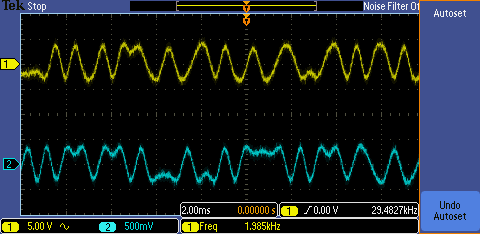
\includegraphics[width=0.65\textwidth]{img/task_a_oscilloscope.png}
    \caption{In-phase and Quadrature component.}
  \end{center}
\end{figure}

\begin{figure}[h]
  \begin{center}
    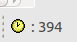
\includegraphics[width=0.65\textwidth]{img/task_a_profile.png}
    \caption{In-phase and Quadrature profile.}
  \end{center}
\end{figure}

\pagebreak
\textbf{Task b)}

\begin{figure}[h]
  \begin{center}
    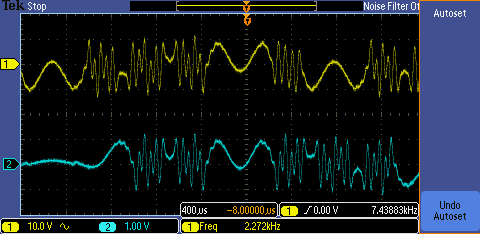
\includegraphics[width=0.65\textwidth]{img/task_b_oscilloscope.png}
    \caption{In-phase and Quadrature component of PN sequence.}
  \end{center}
\end{figure}

\begin{figure}[h]
  \begin{center}
    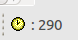
\includegraphics[width=0.65\textwidth]{img/task_b_profile.png}
    \caption{In-phase and Quadrature profile of PN sequence.}
  \end{center}
\end{figure}

\pagebreak
\textbf{Task c)}

\begin{figure}[h]
  \begin{center}
    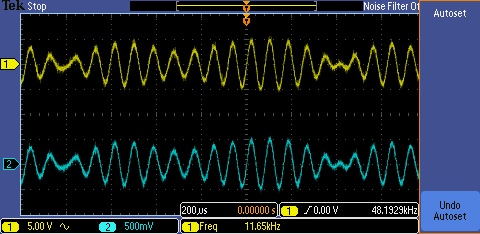
\includegraphics[width=0.65\textwidth]{img/task_c_oscilloscope.png}
    \caption{In-phase and Quadrature component of optimized pulse shape.}
  \end{center}
\end{figure}

\begin{figure}[h]
  \begin{center}
    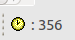
\includegraphics[width=0.65\textwidth]{img/task_c_profile.png}
    \caption{In-phase and Quadrature profile of optimized pulse shape.}
  \end{center}
\end{figure}

\pagebreak
\textbf{Task d)}

\begin{figure}[h]
  \begin{center}
    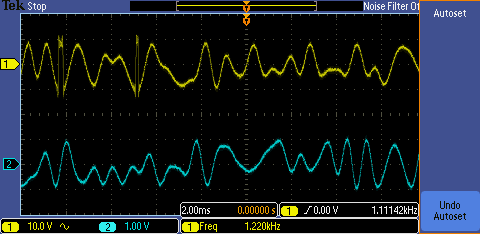
\includegraphics[width=0.65\textwidth]{img/task_d_oscilloscope.png}
    \caption{In-phase and Quadrature component of 16-QAM.}
  \end{center}
\end{figure}

\begin{figure}[h]
  \begin{center}
    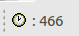
\includegraphics[width=0.65\textwidth]{img/task_d_profile.png}
    \caption{In-phase and Quadrature component of 16-QAM PN sequence.}
  \end{center}
\end{figure}

\pagebreak
\textbf{Code: 16-QAM}

\begin{verbatim}

	// left (quadrature), right (in-phase)
	const float QPSK_LUT[16][2] = {
	{     -3 * QPSK_SCALE,  -3 * QPSK_SCALE}, /* QPSK_LUT[0]  */
	{     -3 * QPSK_SCALE, -1 * QPSK_SCALE}, /* QPSK_LUT[1]  */
	{    -3 * QPSK_SCALE,  3 * QPSK_SCALE}, /* QPSK_LUT[2]  */
	{    -3 * QPSK_SCALE,  1 * QPSK_SCALE}, /* QPSK_LUT[3]  */
	{    -1 * QPSK_SCALE, -3 * QPSK_SCALE}, /* QPSK_LUT[4]  */
	{    -1 * QPSK_SCALE, -1 * QPSK_SCALE}, /* QPSK_LUT[5]  */
	{    -1 * QPSK_SCALE,  3 * QPSK_SCALE}, /* QPSK_LUT[6]  */
	{    -1 * QPSK_SCALE,  1 * QPSK_SCALE}, /* QPSK_LUT[7]  */
	{     3 * QPSK_SCALE, -3 * QPSK_SCALE}, /* QPSK_LUT[8]  */
	{     3 * QPSK_SCALE, -1 * QPSK_SCALE}, /* QPSK_LUT[9]  */
	{     3 * QPSK_SCALE,  3 * QPSK_SCALE}, /* QPSK_LUT[10]  */
	{     3 * QPSK_SCALE,  1 * QPSK_SCALE}, /* QPSK_LUT[11]  */
	{     1 * QPSK_SCALE, -3 * QPSK_SCALE}, /* QPSK_LUT[12]  */
	{     1 * QPSK_SCALE, -1 * QPSK_SCALE}, /* QPSK_LUT[13]  */
	{     1 * QPSK_SCALE,  3 * QPSK_SCALE}, /* QPSK_LUT[14]  */
	{     1 * QPSK_SCALE, -1 * QPSK_SCALE}, /* QPSK_LUT[15]  */
	};

	/************************************************************/
	// I added my impulse modulated QPSK routine here
	if (counter == 0) {
		symbol = rand() & 0xF;

		xI[0]  = QPSK_LUT[symbol][RIGHT];  
		xQ[0]  = QPSK_LUT[symbol][ LEFT];   
	}

	// perform impulse modulation based on the FIR filter, B[N]
	yI = 0;
	yQ = 0;

	for (i = 0; i < span; i++) {
		// perform the "I" dot-product
		yI += xI[i]*pulse[counter + samplesPerSymbol*i];	

		// perform the "Q" dot-product
		yQ += xQ[i]*pulse[counter + samplesPerSymbol*i];	
	}

	if (counter >= (samplesPerSymbol - 1)) {
		counter = -1; 

		/* shift xI[] and xQ[] in preparation to receive the next input */
		for (i = 5; i > 0; i--) {
			// setup xI[] for the next input value
			xI[i] = xI[i-1];  

			// setup xQ[] for the next input value
			xQ[i] = xQ[i-1];  
		}
	}

	counter++;

	output = output_gain*(yI*cosine[counter & 3] - yQ*sine[counter & 3]);
\end{verbatim}

\pagebreak
\textbf{Task e)}

\begin{figure}[h]
  \begin{center}
    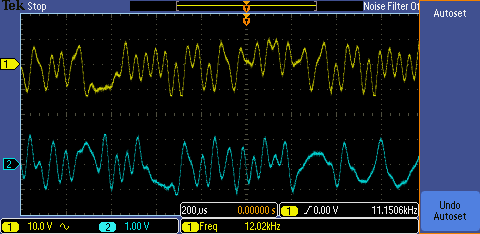
\includegraphics[width=0.65\textwidth]{img/task_e_oscilloscope.png}
    \caption{In-phase and Quadrature component of PN sequence.}
  \end{center}
\end{figure}

\begin{figure}[h]
  \begin{center}
    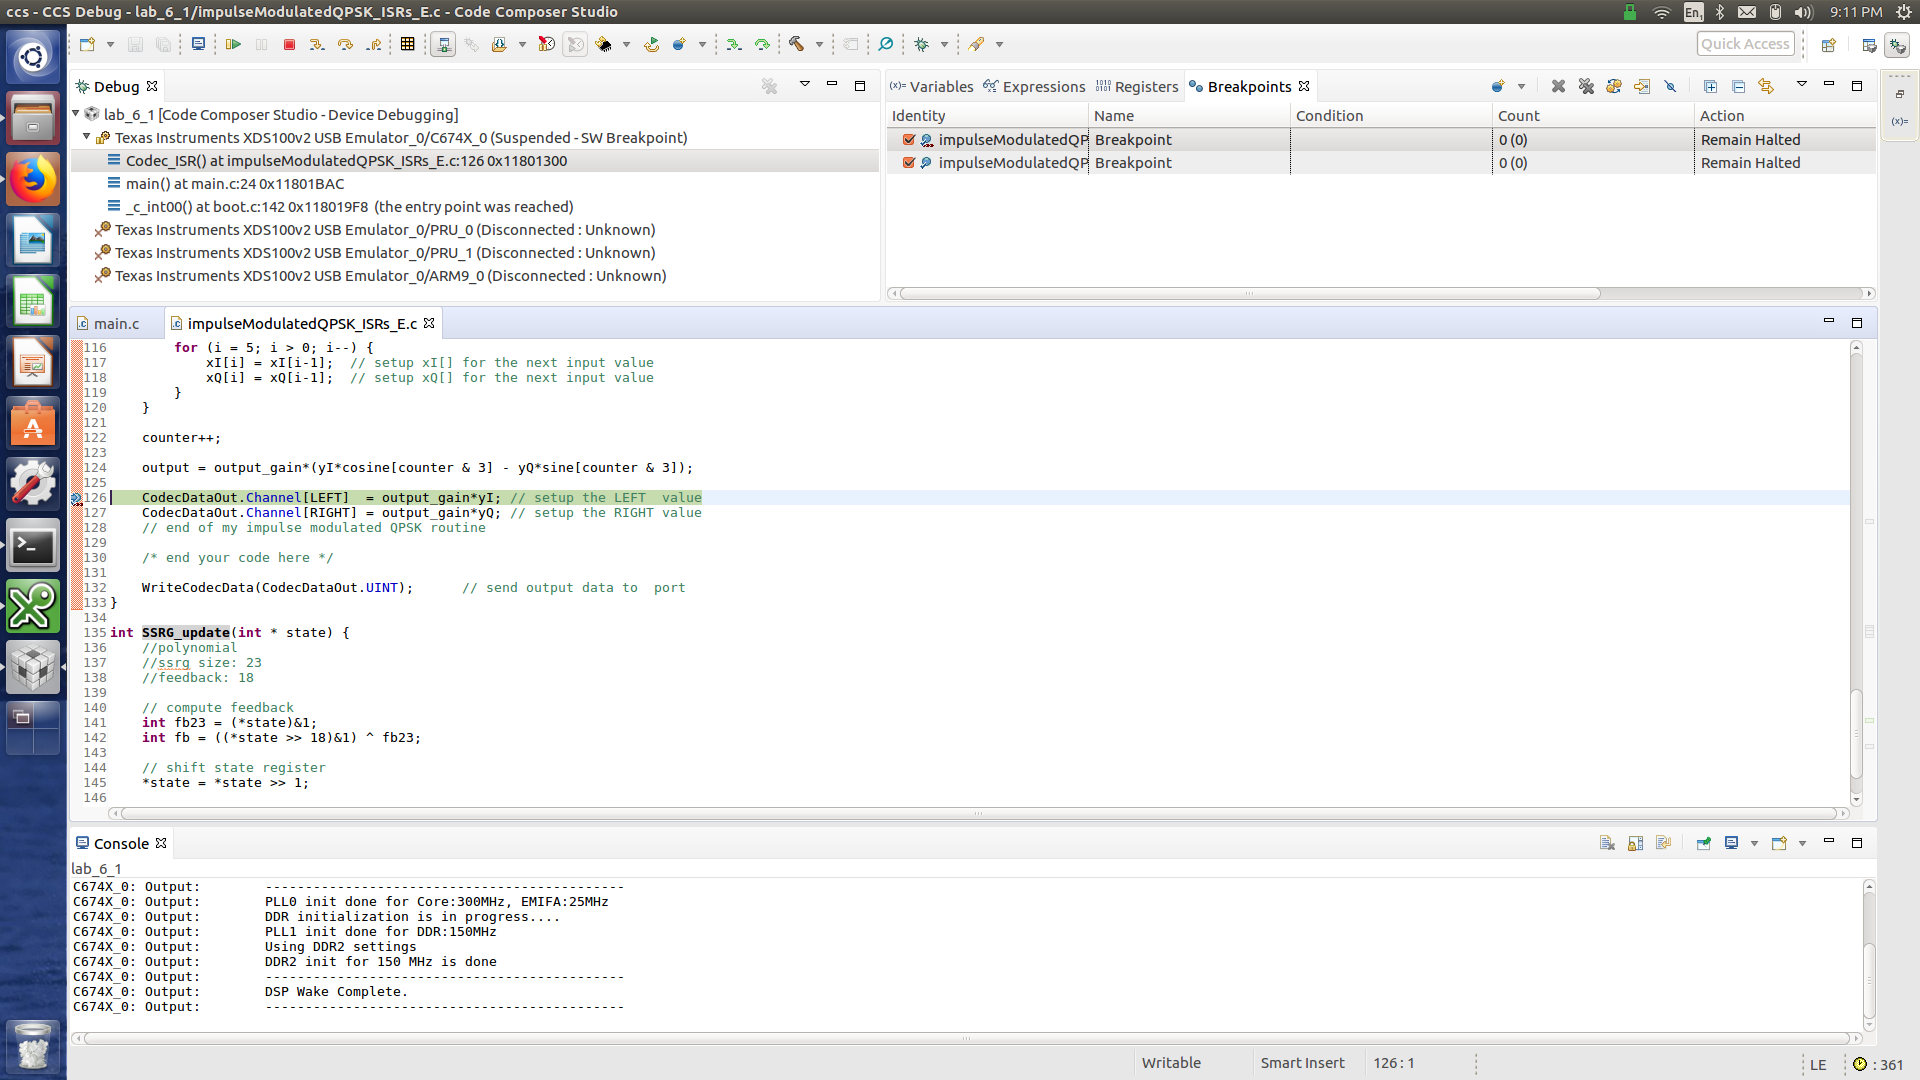
\includegraphics[width=0.65\textwidth]{img/task_e_profile.png}
    \caption{In-phase and Quadrature component of PN sequence.}
  \end{center}
\end{figure}

\pagebreak
\textbf{Code: 16-QAM with PN sequence}

\begin{verbatim}

	// left (quadrature), right (in-phase)
	const float QPSK_LUT[16][2] = {
	{     -3 * QPSK_SCALE,  -3 * QPSK_SCALE}, /* QPSK_LUT[0]  */
	{     -3 * QPSK_SCALE, -1 * QPSK_SCALE}, /* QPSK_LUT[1]  */
	{    -3 * QPSK_SCALE,  3 * QPSK_SCALE}, /* QPSK_LUT[2]  */
	{    -3 * QPSK_SCALE,  1 * QPSK_SCALE}, /* QPSK_LUT[3]  */
	{    -1 * QPSK_SCALE, -3 * QPSK_SCALE}, /* QPSK_LUT[4]  */
	{    -1 * QPSK_SCALE, -1 * QPSK_SCALE}, /* QPSK_LUT[5]  */
	{    -1 * QPSK_SCALE,  3 * QPSK_SCALE}, /* QPSK_LUT[6]  */
	{    -1 * QPSK_SCALE,  1 * QPSK_SCALE}, /* QPSK_LUT[7]  */
	{     3 * QPSK_SCALE, -3 * QPSK_SCALE}, /* QPSK_LUT[8]  */
	{     3 * QPSK_SCALE, -1 * QPSK_SCALE}, /* QPSK_LUT[9]  */
	{     3 * QPSK_SCALE,  3 * QPSK_SCALE}, /* QPSK_LUT[10]  */
	{     3 * QPSK_SCALE,  1 * QPSK_SCALE}, /* QPSK_LUT[11]  */
	{     1 * QPSK_SCALE, -3 * QPSK_SCALE}, /* QPSK_LUT[12]  */
	{     1 * QPSK_SCALE, -1 * QPSK_SCALE}, /* QPSK_LUT[13]  */
	{     1 * QPSK_SCALE,  3 * QPSK_SCALE}, /* QPSK_LUT[14]  */
	{     1 * QPSK_SCALE, -1 * QPSK_SCALE}, /* QPSK_LUT[15]  */
	};

	/************************************************************/
	// I added my impulse modulated QPSK routine here
	if (counter == 0) {
		/* generate 2 random bits */
		symbol = SSRG_update(&SSRG_state); 
		symbol = (symbol << 1) + SSRG_update(&SSRG_state);
		symbol = (symbol << 1) + SSRG_update(&SSRG_state);
		symbol = (symbol << 1) + SSRG_update(&SSRG_state);

		xI[0]  = QPSK_LUT[symbol][RIGHT];  
		xQ[0]  = QPSK_LUT[symbol][ LEFT];   
	}

	// perform impulse modulation based on the FIR filter, B[N]
	yI = 0;
	yQ = 0;

	for (i = 0; i < span; i++) {
		// perform the "I" dot-product
		yI += xI[i]*pulse[counter + samplesPerSymbol*i];	

		// perform the "Q" dot-product
		yQ += xQ[i]*pulse[counter + samplesPerSymbol*i];	
	}

	if (counter >= (samplesPerSymbol - 1)) {
		counter = -1; 

		/* shift xI[] and xQ[] in preparation to receive the next input */
		for (i = 5; i > 0; i--) {
			// setup xI[] for the next input value
			xI[i] = xI[i-1];  

			// setup xQ[] for the next input value
			xQ[i] = xQ[i-1];  
		}
	}

	counter++;

	output = output_gain*(yI*cosine[counter & 3] - yQ*sine[counter & 3]);
\end{verbatim}

\pagebreak
\textbf{Task 2b)}

\begin{figure}[h]
  \begin{center}
    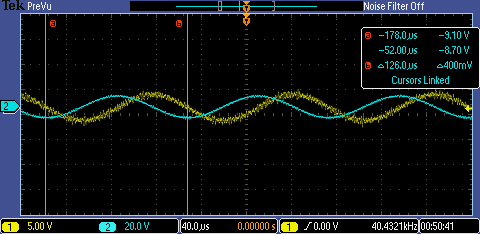
\includegraphics[width=0.65\textwidth]{img/task_2_b_oscilloscope.png}
    \caption{8kHz carrier wave.}
  \end{center}
\end{figure}

\begin{figure}[h]
  \begin{center}
    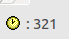
\includegraphics[width=0.65\textwidth]{img/task_2_b_profile.png}
    \caption{8kHz carrier wave profile.}
  \end{center}
\end{figure}

\pagebreak
\textbf{Task 2c)}

\begin{figure}[h]
  \begin{center}
    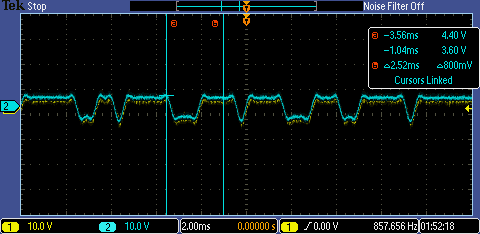
\includegraphics[width=0.65\textwidth]{img/task_2_c_oscilloscope.png}
    \caption{Demodulated in-phase component.}
  \end{center}
\end{figure}

\begin{figure}[h]
  \begin{center}
    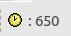
\includegraphics[width=0.65\textwidth]{img/task_2_c_profile.png}
    \caption{Demodulated in-phase profile.}
  \end{center}
\end{figure}

\pagebreak
\textbf{Task 2d)}

\begin{figure}[h]
  \begin{center}
    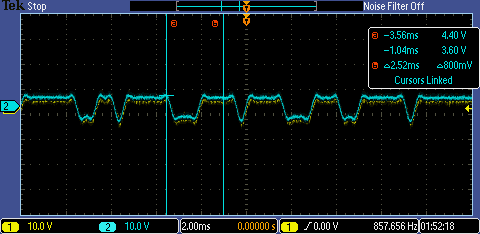
\includegraphics[width=0.65\textwidth]{img/task_2_c_oscilloscope.png}
    \caption{Demodulated quadrature component.}
  \end{center}
\end{figure}

\begin{figure}[h]
  \begin{center}
    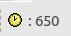
\includegraphics[width=0.65\textwidth]{img/task_2_c_profile.png}
    \caption{Demodulated quadrature profile.}
  \end{center}
\end{figure}

\pagebreak
\textbf{Code: Reciever Demodulation}

\begin{verbatim}
	// I added my impulse modulated QPSK routine here
	if (counter == 0) {
		/* generate 2 random bits */
		symbol = SSRG_update(&SSRG_state); 
		symbol = (symbol << 1) + SSRG_update(&SSRG_state);

		xI[0]  = QPSK_LUT[symbol][RIGHT];  
		xQ[0]  = QPSK_LUT[symbol][ LEFT];   
	}

	// perform impulse modulation based on the FIR filter, B[N]
	yI = 0;
	yQ = 0;

	for (i = 0; i < span; i++) {
		// perform the "I" dot-product
		yI += xI[i]*pulse[counter + samplesPerSymbol*i];	

		// perform the "Q" dot-product
		yQ += xQ[i]*pulse[counter + samplesPerSymbol*i];	
	}

	if (counter >= (samplesPerSymbol - 1)) {
		counter = -1; 

		/* shift xI[] and xQ[] in preparation to receive the next input */
		for (i = 5; i > 0; i--) {
			// setup xI[] for the next input value
			xI[i] = xI[i-1];  

			// setup xQ[] for the next input value
			xQ[i] = xQ[i-1];  
		}
	}

	counter++;
	carrier_index = (carrier_index + 1) % 6;

	output = output_gain*(yI*cosine[carrier_index] - yQ*sine[carrier_index]);
	// end of my impulse modulated QPSK routine

	//demodulate in-phase and quadrature
  float demod_inphase = 2*output*cosine[carrier_index];
  float demod_quad = -2*output*sine[carrier_index];

  //LPF
  biquad_x_inphase[0][0] = demod_inphase;
  biquad_x_quad[0][0] = demod_quad;

  float output_inphase = G[0] * biquad_inphase(0, biquad_x_inphase[0][0]);
  float output_quad = G[0] * biquad_quadrature(0, biquad_x_quad[0][0]);
\end{verbatim}

%----------------------------------------------------------------------------------------
%	SECTION 4
%----------------------------------------------------------------------------------------

\section{Discussion}

\subsection{Pulse Shaping}


%----------------------------------------------------------------------------------------
%	SECTION 5
%----------------------------------------------------------------------------------------

\section{Answers to questions}

\begin{enumerate}
  \begin{item}
    Explain why we changed the carrier frequency to properly simulate the receiver. 

  \textbf{Answer:}
    The sampling rate of the DSP board is set to 48kHz so the maximum frequency that we can represent is 24kHz.
    If we kept the the frequency of the carrier at 12kHz, then when we demodulated we would have a sinusoid alias to DC
    because we would get the original baseband signal plus a sinusoid with twice the carrier frequency.
  \end{item}

  \begin{item}
    Explain your choice of cutoff frequency for the demodulation filter.

  \textbf{Answer:}
    The cutoff must be equal to the bandwidth of the baseband signal, but less than twice the carrier frequency.
  \end{item}

  \begin{item}
    The QAM signal can be viewed as the sum of two PAM signals that each have been modulated by a carrier. How is the bandwidth of the QAM signal related to the bandwidth of its two (carrier-modulated) PAM components?

  \textbf{Answer:}
    QAM encodes information in both the amplitude and phase of the carrier, where as PAM only encodes information in the amplitude of the carrier.
    So PAM takes twice the bandwidth of QAM.

  \end{item}
\end{enumerate}

\end{document}
